% Included from both -slides and -handout versions.
\documentclass[pdftex]{beamer} % used to trigger beamer mode in Emacs,
                               % normally commented out.

\usetheme{metropolis}

\usepackage[english]{babel}
\usepackage[latin1]{inputenc}
\usepackage{graphicx}
\usepackage{times}
\usepackage[T1]{fontenc}
\usepackage{fancyvrb}
\usepackage{listings}
\begin{document}
\lstset{language=C, escapeinside={(*@}{@*)}, numbers=left,
  basicstyle=\tiny, showspaces=false, showtabs=false}

\title{Introduction to Operating Systems}
\subtitle{Through tracing, analysis, and experimentation}
%\institute{University of Cambridge}
\author{George V. Neville-Neil \& Dr Robert N. M. Watson}
\date{8 August 2016}

\begin{frame}
  \titlepage
\end{frame}

\section{Course Overview}

\begin{frame}
  \frametitle{Course Goals}
  \begin{itemize}
  \item A grounding in systems principles
  \item A grand tour of the Operating System
  \item Practical insights into how the OS works
  \end{itemize}
\end{frame}

\begin{frame}
  \frametitle{Course Outline}
  \begin{description}
  \item[Monday] Overview and Introdcution
    \begin{itemize}
    \item High Level Definitions
    \item History
    \item Introduction to Tracing
    \item Lab 1: System Setup and First Traces
    \end{itemize}
  \item[Tuesday] Processing Data
    \begin{itemize}
    \item Quiz
    \item Processes 
    \item Locking
    \item Scheduling
    \item Virtual Memory
    \item Lab 2: Tracking Processes
    \end{itemize}
  \end{description}
\end{frame}

\begin{frame}
  \frametitle{Course Outline}
  \begin{description}
  \item[Wednesday] Communication
    \begin{itemize}
    \item I/O
    \item Inter Process Communication
    \item Sockets and Network Communication
    \item Lab 3: TCP Connection Setup
    \end{itemize}
  \item[Thursday] Storing Data
    \begin{itemize}
    \item Storage Overview
    \item Naming and Location
    \item Virtual Filesystem Layer
    \item Storing and Retrieving Data
    \item Lab 4: Reading a file from disk
    \end{itemize}
  \end{description}
\end{frame}

\begin{frame}
  \frametitle{Course Outline}
  \begin{description}
  \item[Friday] Whole System View
    \begin{itemize}
    \item Serving Web Content
    \item NGINX
    \item Review
    \item Final Exam
    \end{itemize}
  \end{description}
\end{frame}

\begin{frame}
  \frametitle{Lab Work}
  \begin{description}
  \item [Tracing] Systems Setup, Begin using DTrace
  \item [Processes] Tracing the Process Life Cycle
  \item [Communication] Networking and TCP
  \item [Storage] Storing and Retrieving Data
  \end{description}
\end{frame}

\begin{frame}
  \frametitle{Day Plan}
  \begin{tabular*}{1.0\linewidth}{l|l}
    Time & Topic \\
    \hline
    09:15-09:45 & \textbf{Overview} \\
    09:45-10:00 & Break \\
    10:00-12:00 & What is an Operating System? \\
    12:00-13:00 & Lunch \\
    13:00-14:15 & Introduction to DTrace and Tracing \\
    14:15-14:30 & Break \\
    14:30-16:30 & Lab 1 \\
    16:30-17:00 & Lab 1 Review
  \end{tabular*}
\end{frame}

\section{High Level Overview}
\begin{frame}
  \frametitle{What do computers do?}
  \begin{description}
  \item[Processing] Converting information from one form to another.
  \item[Communication] Moving information between one or more systems.
  \item[Storage] Maintaining information over time.
  \end{description}
\end{frame}

\begin{frame}
  \frametitle{What is an Operating System?}
  \begin{center}
    \begin{itemize}
    \item \emph{White Boarding Exercise.}
    \end{itemize}
  \end{center}
\end{frame}

\begin{frame}
  \frametitle{What an Operating System Does}
  \begin{itemize}
  \item Provides the \emph{Programming Model}

\pause

  \item Protects Programs from each other

\pause

  \item Controls access to hardware

\pause

  \item Ensures fair sharing of resources
  \end{itemize}
\end{frame}

\begin{frame}[fragile]
  \frametitle{What an Operating System Is}
  \begin{itemize}
  \item A single large program
  \item Written in the C language
  \item Built with \texttt{make}
  \item More than $20,000$ files
  \item $12,000,000$ lines of code
  \end{itemize}
\end{frame}

\section{History: How did we get here?}

\begin{frame}
  \frametitle{Computer History from the Operating System Perspective}
  \begin{description}
  \item [The Hardware Environment] Defines what is possible.
  \item [Requirements] What are we asking the system to do?
  \item [Services] What can the OS provide.
  \end{description}
\end{frame}

\begin{frame}
  \frametitle{In the beginning: early computers}
  \begin{itemize}
  \item Wired programs
  \item Highly specialized to only one problem
  \item Armies of programmers tend a single machine
  \end{itemize}
\end{frame}

\begin{frame}
  \frametitle{The First Programmers}
  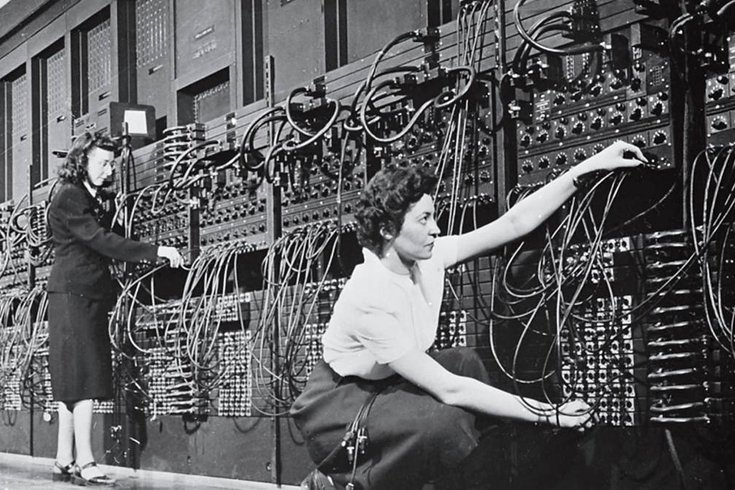
\includegraphics[width=\textwidth]{../../figures/first_programmers.jpg}
\end{frame}

\begin{frame}
  \frametitle{Early Computers}
  \begin{itemize}
  \item Processing measured in hundres of Hz
  \item Tiny memories
  \item Limited to no input/output devices
  \item Not much for an Operating System to do or provide
  \end{itemize}
\end{frame}

\begin{frame}
  \frametitle{Mainframes and Batch Processing}
  \begin{itemize}
  \item Standardized input/output with cards
  \item One program at a time (batch processing)
  \item No interactive programming
  \item Early disks and printers
  \item What is a byte?
  \item The rise of computer languages.
  \item Earliest operating systems (monitors)
  \end{itemize}
\end{frame}

\begin{frame}
  \frametitle{5Mb of Source Code}
  \centering
  \includegraphics[width=0.5\textwidth]{../../figures/punched-cards-5mb.jpg}  
\end{frame}

\begin{frame}
  \frametitle{Mini-computers and Time Sharing Systems}
  \begin{itemize}
  \item Shrinking hardware and affordable computing resources
  \item CTSS
  \item MULTICS
  \item C, the portable assembler
  \item UNIX
  \item (D)ARPANet
  \end{itemize}
\end{frame}

\begin{frame}
  \frametitle{The UNIX Kernel}
\centering
  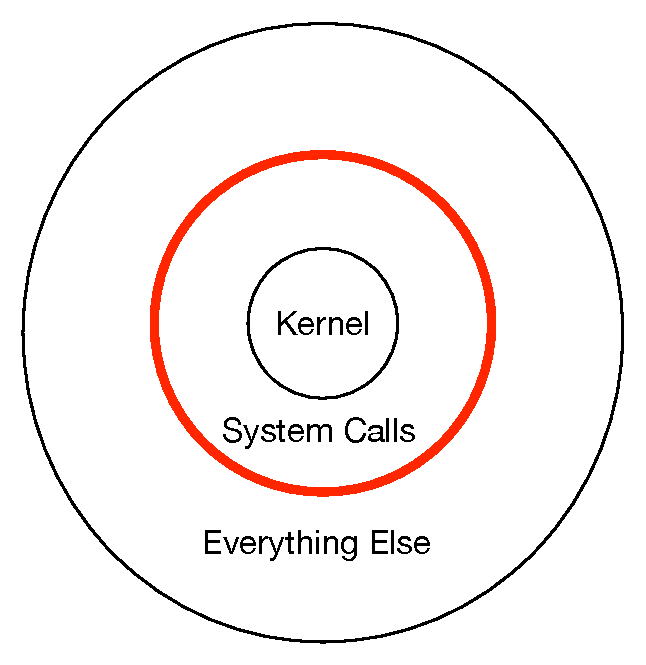
\includegraphics[width=0.5\textwidth]{../../figures/simplified-kernel.pdf}  
\end{frame}

\begin{frame}
  \frametitle{The Rise of the Microcomputer}
  \begin{itemize}
  \item LSI shrinks hardware onto the first chip based processors
  \item Moore's Law
  \item Less powerful than mini-computers
  \item 8-bitting
  \item Single user
  \item No networking
  \item Operating System is a monitor and convience routines
  \end{itemize}
\end{frame}

\begin{frame}
  \frametitle{Home Microcomputer}
  \centering
  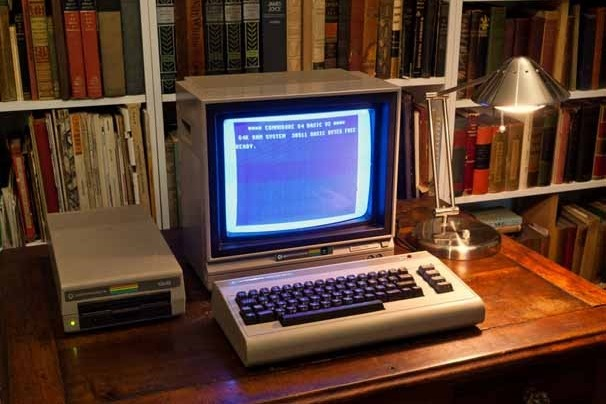
\includegraphics[width=\textwidth]{../../figures/c64.jpg}  
\end{frame}

\begin{frame}
  \frametitle{Workstations and Networking}
  \begin{itemize}
  \item VLSI provides faster and more powerful CPUs
  \item Graphical Displays (X10 and X11)
  \item Ethernet
  \item TCP/IP
  \item UNIX is the de-facto standard, sort of
  \end{itemize}
\end{frame}

\begin{frame}
  \frametitle{Workstation}
  \centering
  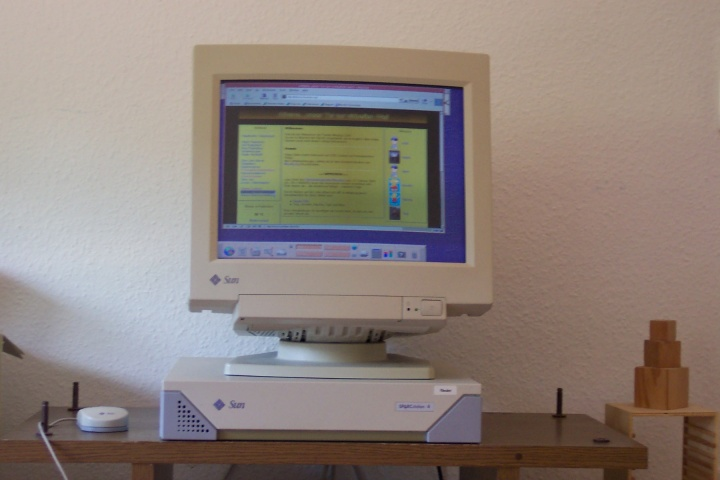
\includegraphics[width=\textwidth]{../../figures/workstation.jpg}  
\end{frame}

\begin{frame}
  \frametitle{Embedded and Real Time}
  \begin{itemize}
  \item Applied kernel programming
  \item Tasks have deadlines
  \item Failure is not an option
  \item Often forgo more expensive UNIX like features
  \end{itemize}
\end{frame}

\begin{frame}
  \frametitle{Mobile Devices and the Ubiquitous Internet}
  \begin{itemize}
  \item Sensors
  \item Always connected
  \item A return to single user, but with a multi-user OS
  \item Programming for power rather than speed
  \end{itemize}
\end{frame}

\begin{frame}
  \frametitle{The Present Day}
  \begin{itemize}
  \item Multi-user Unix like systems everywhere
  \item Continued use of C for OS development
  \item Heterogenous environments
  \end{itemize}
\end{frame}

\section{Example System}
\label{sec:example-system}

\begin{frame}
  \frametitle{Our Challenge}
  \begin{itemize}
  \item How does data move in a real world system?
  \item Serving Data from Storage to Clients
    \begin{description}
    \item[Program] Web Server
    \item[Stored Data] Filesystem
    \item[Communication] Network Stack
    \end{description}
  \end{itemize}
\end{frame}

\begin{frame}
  \frametitle{UNIX Philosophies}
  \begin{itemize}
  \item Everything is a byte stream
  \item Do a small number of things well
  \item Build complex systems out of simple building blocks
  \item Swiss Army Knife vs. Toolbox
  \end{itemize}
\end{frame}

\begin{frame}
  \frametitle{Special Considerations}
  \begin{itemize}
  \item An OS kernel is one, large program.
  \item More than $50,000$ functions.
  \item $5677$ files    
  \item $5,131,552$ lines of C code.
  \item A unique programming environment
  \end{itemize}
\end{frame}

\begin{frame}
  \frametitle{Design and Implementation Requirements}
  \begin{description}
  \item[Fast] Low overhead, high performaance
  \item[Safe] Secure, tractable
  \item[Flexible] Can be used by many applications
  \end{description}
\end{frame}

\begin{frame}
  \frametitle{Operating System: The Unix View}
  
\end{frame}

\begin{frame}[fragile]
  \frametitle{User vs. Kernel Space}
  \begin{columns}[t]
    \begin{column}{5cm}
      \emph{User Space}
      \begin{itemize}
      \item User Programs
      \item Libraries
      \item All memory is \emph{virtual}
      \item A world of illusions
      \end{itemize}
    \end{column}
    \begin{column}{5cm}
      \emph{Kernel Space}
      \begin{itemize}
      \item Device Drivers
      \item Physical Memory
      \item Cold reality
      \end{itemize}
    \end{column}
  \end{columns}
\end{frame}

\begin{frame}[fragile]
  \frametitle{System Calls: The Operating System's API}
  \begin{itemize}
  \item Border between User and Kernel Space
  \item Everything that \emph{can} be done with the OS
  \item \verb|open()|, \verb|read()|, \verb|write()|, \verb|close()|
  \item Over 1000 separate interfaces
  \item Section 2 of the manual set
  \end{itemize}
\end{frame}

\begin{frame}
  \frametitle{OS Programming}
  \begin{itemize}
  \item C is the lingua franca
  \item Simple data structures
    \begin{itemize}
    \item Lists
    \item Hash Tables
    \end{itemize}
  \item Hand crafted classes and objects
  \item Programming without a net
  \end{itemize}
\end{frame}

\begin{frame}
  \frametitle{Competing Kernel Architectures}
  \begin{columns}[t]
    \begin{column}{5cm}
      \emph{Micro-Kernel}
      \begin{itemize}
      \item Kernel is Only a Scheduler
      \item Services Model
      \item in-kernel IPC
      \item POSIX as a service
      \item Mach, Barrelfish, L4
      \end{itemize}
    \end{column}
    \begin{column}{5cm}
      \emph{Monolithic}
      \begin{itemize}
      \item One big program
      \item Function Calls
      \item System Call API
      \item FreeBSD, Linux, Windows
      \end{itemize}  
    \end{column}
  \end{columns}
\end{frame}

\begin{frame}
  \frametitle{Review: What an Operating System Does}
  \begin{itemize}
  \item Provides the \emph{Programming Model}
  \item Protects Programs from each other
  \item Controls access to hardware
  \item Ensures fair sharing of resources
  \end{itemize}
\end{frame}

\section{Introduction to Tracing}
\label{sec:intro-tracing}

\begin{frame}[fragile]
  \frametitle{History of Debugging}
  \begin{itemize}
  \item Blinking lights
  \item Radio Frequency Interference (AM Radio)
  \item \verb|print| statements
  \item Trace Instructions
  \end{itemize}
\end{frame}

\begin{frame}
  \frametitle{What is DTrace?}
  \begin{itemize}
  \item A dynamic tracing framework for software
  \item Low impact on overall system performance
  \item Does not incur costs when not in use
  \end{itemize}
\end{frame}

\begin{frame}
  \frametitle{What can DTrace show me?}
  \begin{itemize}
  \item When a function is being called
  \item A function's arguments
  \item The frequency of function calls
  \item A whole lot more...
  \end{itemize}
\end{frame}

\begin{frame}[fragile]
  \frametitle{A Simple Example}
  \begin{lstlisting}
dtrace -n syscall:::
dtrace: description 'syscall:::' matched 2148 probes
CPU     ID                    FUNCTION:NAME
  1  51079                     ioctl:return 
  1  51078                      ioctl:entry 
  1  51079                     ioctl:return 
  1  51078                      ioctl:entry 
  1  51079                     ioctl:return 
  1  51632                sigprocmask:entry 
  1  51633               sigprocmask:return 
  1  51784                  sigaction:entry 
  \end{lstlisting}
  \begin{itemize}
  \item Look at all system calls
  \end{itemize}
\end{frame}

\begin{frame}
  \frametitle{How does DTrace Work?}
  \begin{itemize}
  \item Various probes are added to the system
  \item The probes are activated using the dtrace program
  \item A small number of assembly instructions are modified at
    run-time to get the system to run in the probe
  \end{itemize}
\end{frame}

\begin{frame}[fragile]
  \frametitle{A more complex example}
\begin{lstlisting}
dtrace -n 'syscall::write:entry /arg2 != 0/ { printf("write size % d\n", arg2); } '
dtrace: description 'syscall::write:entry ' matched 2 probes
CPU     ID                    FUNCTION:NAME
0  50978                      write:entry write size 1
0  50978                      write:entry write size 55
0  50978                      write:entry write size 2
\end{lstlisting}
\end{frame}

\begin{frame}[fragile]
  \frametitle{DTrace Glossary}
  \begin{description}
  \item[Probe] A way of specifying what to trace
  \item[Provider] A DTrace defined module that provides information
    about something in the system
  \item[Module] A software module, such as \Verb+kernel+
  \item[Function] A function in a module, such as \Verb+ether_input+
  \item[Predicate] A way of filtering DTrace probes
  \item[Action] A set of D language statements carried out when a probe
    is matched
  \end{description}
\end{frame}

\begin{frame}
  \frametitle{Providers}
  \begin{description}
  \item[fbt] Function Boundary Tracing ($50413$)
  \item[syscall] System Calls ($2148$)
  \item[profile] Timing source 
  \item[proc] Process Operations 
  \item[sched] Scheduler
  \item[io] I/O calls
  \item[ip] Internet Protocol
  \item[udp] UDP
  \item[tcp] TCP
  \item[vfs] Filesystem Routines
  \end{description}
\end{frame}

\begin{frame}[fragile]
  \frametitle{Dissecting a Probe}
  \begin{itemize}
  \item \Verb+syscall::write:entry+
    \begin{description}
    \item[Provider] syscall
    \item[Module] None
    \item[Function] write
    \item[Name] entry
    \end{description}
  \item \Verb+fbt:kernel:ether_input:entry+
    \begin{description}
    \item[Provider] fbt
    \item[Module] kernel
    \item[Function] \Verb+ether_input+
    \item[Name] entry
    \end{description}
  \end{itemize}
\end{frame}

\begin{frame}
  \frametitle{DTrace Requirements}
  \begin{itemize}
  \item A kernel with DTrace support built in
    \begin{itemize}
    \item Default on FreeBSD 10 or later
    \end{itemize}
  \item The ability to sudo or be root
  \item The complete command syntax is covered in the dtrace manual page
  \end{itemize}
\end{frame}

\begin{frame}[fragile]
  \frametitle{Finding Probes}
  \begin{itemize}
  \item Listing all the probes gets you $50000$ to choose from
  \item Judicious use of providers, modules and grep 
  \item e.g. \Verb+dtrace -l -P syscall+
  \end{itemize}
\end{frame}

\begin{frame}[fragile]
  \frametitle{Probe Arguments}
  \begin{itemize}
  \item Use verbose (-v) mode to find probe arguments
  \item \Verb+sudo dtrace -lv -f syscall:freebsd:read+
  \end{itemize}
\begin{verbatim}
 ID   PROVIDER            MODULE                          FUNCTION NAME
57177    syscall           freebsd                              read entry

	Argument Types
		args[0]: int
		args[1]: void *
		args[2]: size_t
\end{verbatim}
\end{frame}

\begin{frame}
  \frametitle{The D Language}
  \begin{itemize}
  \item A powerful subset of C
  \item Includes features specific to DTrace, such as aggregations
  \item Anything beyond some simple debugging usually required a D
    script
  \end{itemize}
\end{frame}

\begin{frame}[fragile]
  \frametitle{DTrace One-Liners}
  \begin{itemize}
  \item A set of useful single line scripts
  \end{itemize}
\begin{lstlisting}
# Trace file opens with process and filename:
dtrace -n 'syscall::open*:entry { printf("%s %s", execname, copyinstr(arg0)); }'

# Count system calls by program name:
dtrace -n 'syscall:::entry { @[execname] = count(); }'

# Count system calls by syscall:
dtrace -n 'syscall:::entry { @[probefunc] = count(); }'
\end{lstlisting}
\end{frame}

\begin{frame}[fragile]
  \frametitle{Count System Calls}
\begin{lstlisting}
dtrace -n 'syscall:::entry { @[probefunc] = count(); }'
dtrace: description 'syscall:::entry ' matched 1072 probes
^C
 fstat                                                             1
 setitimer                                                         1
 getpid                                                            2
 read                                                              2
 sigreturn                                                         2
 write                                                             3
 getsockopt                                                        4
 select                                                            6
 sigaction                                                         6
 _umtx_op                                                          7
 __sysctl                                                          8
 munmap                                                           18
 mmap                                                             19
 sigprocmask                                                      23
 clock_gettime                                                    42
 ioctl                                                            45
\end{lstlisting}
\end{frame}

\begin{frame}[fragile]
  \frametitle{Aggregations}
  \begin{itemize}
  \item \verb+syscall:::entry { @[probefunc] = count(); }+
  \item The \verb+@[probefunc]+ syntax
  \item Aggregates data during a run for later output
  \item Extremely powerful feature of D language
  \end{itemize}
\end{frame}

\begin{frame}[fragile]
  \frametitle{Quantization}
\begin{lstlisting}
# Summarize requested write() sizes by program name, as power-of-2 distributions (bytes):
dtrace -n 'syscall::write:entry { @[execname] = quantize(arg2); }'
dtrace: description 'syscall::write:entry ' matched 2 probes
^C
  find                                              
           value  ------------- Distribution ------------- count    
               1 |                                         0        
               2 |                                         1        
               4 |                                         17       
               8 |@@                                       841      
              16 |@@@@@@@@@@@@@                            6940     
              32 |@@@@@@@@@@@@@@@@@@@@@@@@@                13666    
              64 |                                         59       
             128 |                                         0        
\end{lstlisting}
\end{frame}

\begin{frame}[fragile]
  \frametitle{Probing the stack}
  \begin{itemize}
  \item Find out how we got where we are
  \item The \verb+stack()+ routine
  \end{itemize}
\end{frame}

\begin{frame}[fragile]
  \frametitle{Who called malloc()?}
\begin{lstlisting}
1  29371                     malloc:entry 
              kernel`cloneuio+0x2c
              kernel`vn_io_fault1+0x3b
              kernel`vn_io_fault+0x18b
              kernel`dofileread+0x95
              kernel`kern_readv+0x68
              kernel`sys_read+0x63
              kernel`amd64_syscall+0x351
              kernel`0xffffffff80d0aa6b
\end{lstlisting}
  \begin{itemize}
  \item Read upwards from the bottom
  \end{itemize}
\end{frame}

\begin{frame}
  \frametitle{DTrace Toolkit}
  \begin{itemize}
  \item An open source set of tools written to use D scripts
  \item Originally specific to Solaris
  \item Exists as a FreeBSD port and package
  \item Currently being updated with new scripts
  \end{itemize}
\end{frame}

\begin{frame}[fragile]
  \frametitle{An example script: hotkernel}
\begin{lstlisting}
./hotkernel 
Sampling... Hit Ctrl-C to end.
^C
FUNCTION                                                COUNT   PCNT
kernel`lookup                                               1   0.1%
kernel`unlock_mtx                                           1   0.1%
kernel`_vm_page_deactivate                                  1   0.1%
...
kernel`amd64_syscall                                        9   0.5%
kernel`pmap_remove_pages                                    9   0.5%
kernel`hpet_get_timecount                                  13   0.7%
kernel`pagezero                                            15   0.8%
kernel`0xffffffff80                                        34   1.9%
kernel`spinlock_exit                                      486  27.0%
kernel`acpi_cpu_c1                                        965  53.6%
\end{lstlisting}
\end{frame}

\begin{frame}[fragile]
  \frametitle{Predicates}
  \begin{itemize}
  \item Filtering probes based on relevant data
  \item Useful for excluding common conditions
  \item \verb+/arg0 != 0/+  Ignore a normal return value
  \end{itemize}
\end{frame}

\begin{frame}[fragile]
  \frametitle{Tracking a Specific Process}
  \begin{itemize}
  \item \verb+pid+ is used to track a Process ID
  \item Used in predicates
  \item \verb+/pid == 1234/+
\end{itemize}
\end{frame}

\begin{frame}[fragile]
  \frametitle{Running a Program Under DTrace}
  \begin{itemize}
  \item DTrace is most often used on running systems
  \item DTrace can be attached at runtime to a program
    \begin{itemize}
    \item \verb+dtrace -p pid ...+
    \end{itemize}
  \item Run a program completely under the control of DTrace
    \begin{itemize}
    \item \verb+dtrace -c cmd ...+
    \end{itemize}
  \end{itemize}
\end{frame}

\begin{frame}
  \frametitle{Going too far}
  \begin{itemize}
  \item Overly broad probes slow down the system
    \begin{itemize}
    \item Watching everything in the kernel
    \item Registering a probe on a module
    \end{itemize}
  \end{itemize}
\end{frame}

\begin{frame}
  \frametitle{The Probe Effect}
  \begin{itemize}
  \item Each probe point has a cost
  \item Every action has a reaction
  \item Any action code requires time to run
  \item Impacts system performance
  \end{itemize}
\end{frame}

\begin{frame}
  \frametitle{Into the Laboratory!}
\end{frame}

\end{document}

%%% Local Variables:
%%% mode: latex
%%% TeX-master: t
%%% End:
